\chapter{Análisis de los resultados}
\label{resultados}

A lo largo de este capitulo se va a tratar de analizar, comparar y discutir los resultados obtenidos mediante HFSS sobre los diseños que se comentaron en la sección \ref{analdis}. Se analizará cada configuración por separado y se mostrarán las gráficas y valores principales para cada una de las configuraciones de 2GHz y 6 GHz y finalmente la configuración a 27 GHz. No se analizará el caso del parche simple a 2.4 GHz puesto que ya fue analizado detalladamente en la sección \ref{procesodiseno}.

\section{Parche Simple a 6 GHz}
\par Para el parche simple a 6 GHz los resultados obtenidos son los siguientes:

\subsection{Pérdidas de retorno}
\par Comenzaremos analizando la curva de pérdidas de retorno o parámetro S del parche simple a 6 GHz, donde se puede observar un valor pico de -40.35 dB y un ancho de banda de 168 MHz, desde los 5.917 GHz hasta los 6.086 GHz, lo que equivale a un 2.81\% de la frecuencia de trabajo.
\\
\begin{figure}[H]
    \centering
        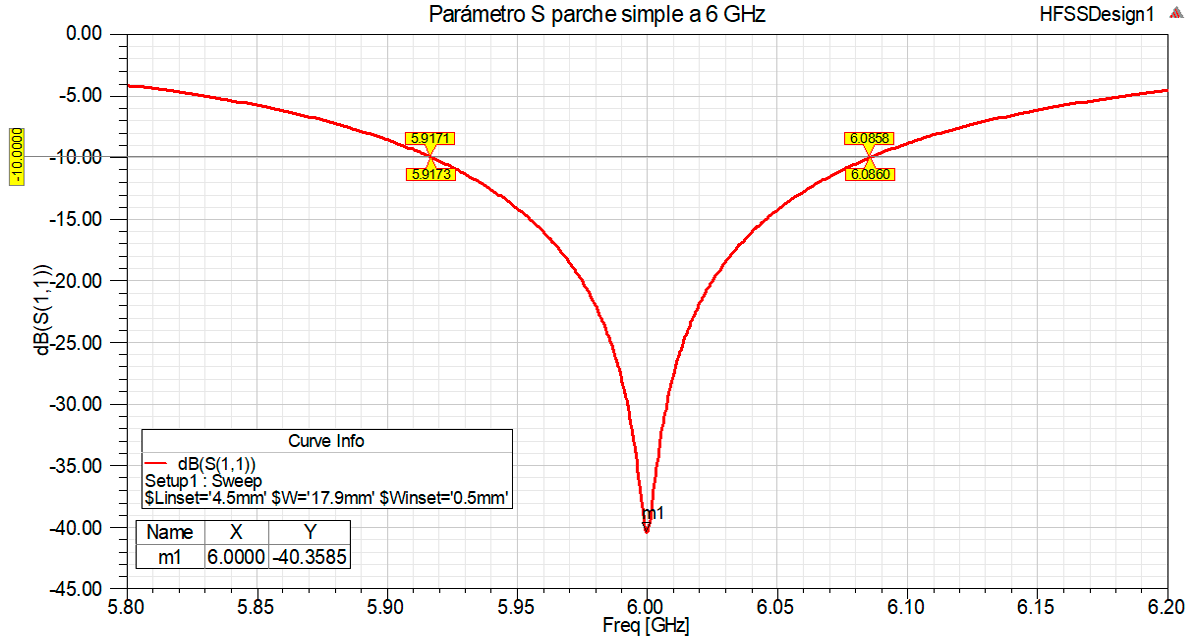
\includegraphics[width=\textwidth]{archivos/analisis/1x12/1}
        \caption{Parámetro S para el parche simple a 6 GHz}
        \label{fig:s1x12}
\end{figure}

\subsection{Reactancia}
\par La curva de reactancia arroja un valor a la frecuencia de trabajo de -0.6 $\Omega$. Muy cerca del valor esperado, 0.
\\
\begin{figure}[H]
    \centering
        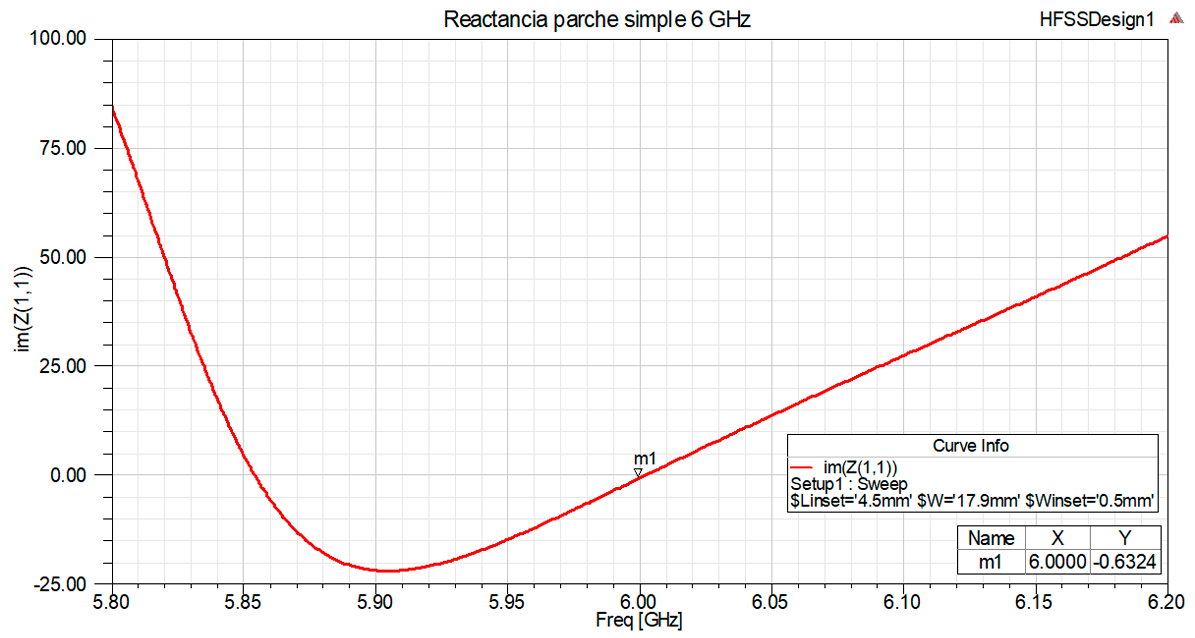
\includegraphics[width=\textwidth]{archivos/analisis/1x12/2}
        \caption{Reactancia para el parche simple a 6 GHz}
        \label{fig:react1x12}
\end{figure}

\subsection{Resistencia}
\par La parte real de la impedancia ofrece un valor a la frecuencia de trabajo de 49.28 $\Omega$. Muy cerca del valor esperado, 50, con un error de tan solo el 1.44\%.
\\
\begin{figure}[H]
    \centering
        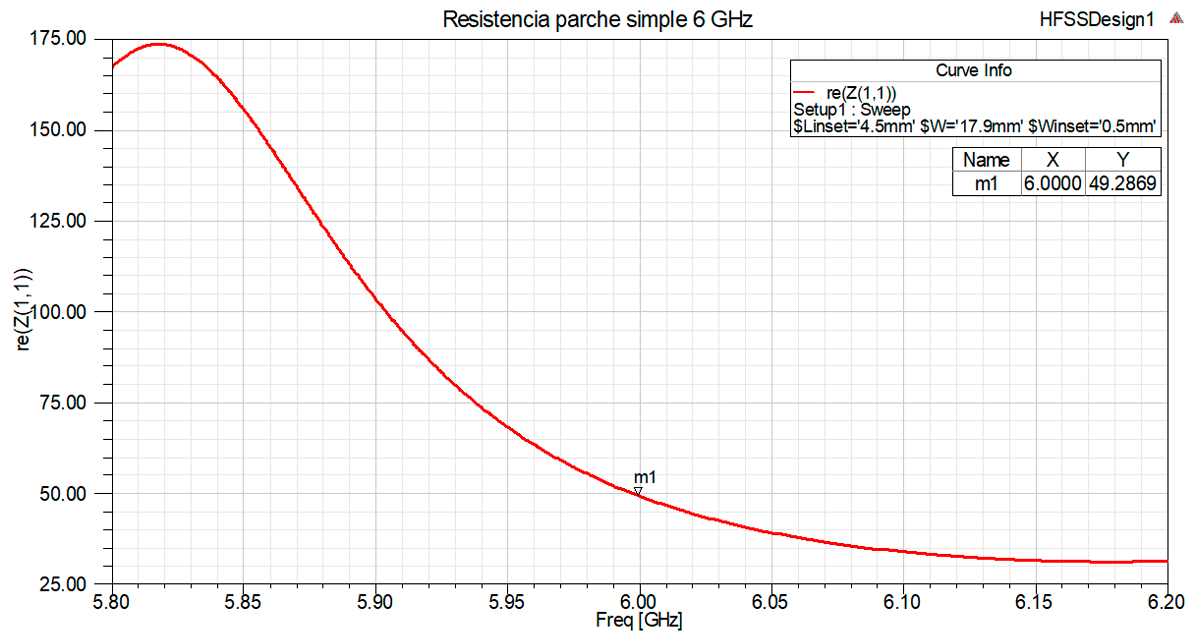
\includegraphics[width=\textwidth]{archivos/analisis/1x12/3}
        \caption{Resistencia para el parche simple a 6 GHz}
        \label{fig:resis1x12}
\end{figure}

\subsection{Patrón de radiación}
\par En cuanto a los patrones de radiación, se puede observar como, al igual que el parche simple a 2.4 GHz, el patrón de radiación es omnidireccional para el plano superior de la antena, y no se ve afectado por ningún otro tipo de elemento radiante. La directividad para el ángulo de máxima radiación encontrada es de 7.66 dB.
\\
\subsubsection{Plano E}
\begin{figure}[H]
    \centering
        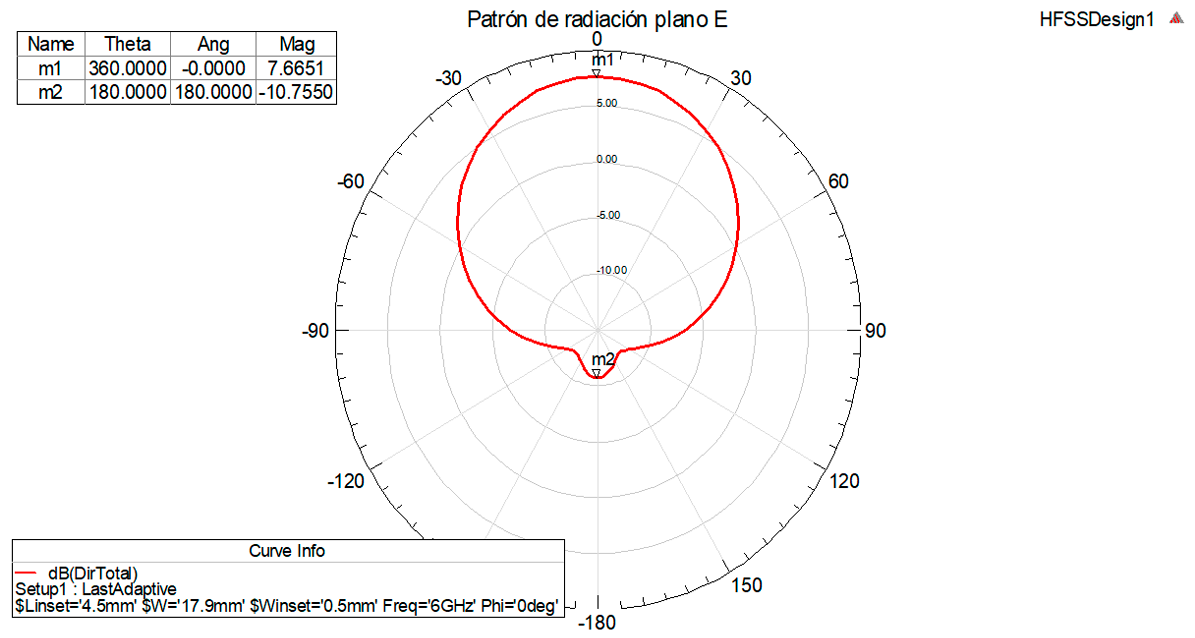
\includegraphics[width=\textwidth]{archivos/analisis/1x12/4}
        \caption{Radiación en el plano E para el parche simple a 6 GHz}
        \label{fig:E1x12}
\end{figure}

\subsubsection{Plano H}
\begin{figure}[H]
    \centering
        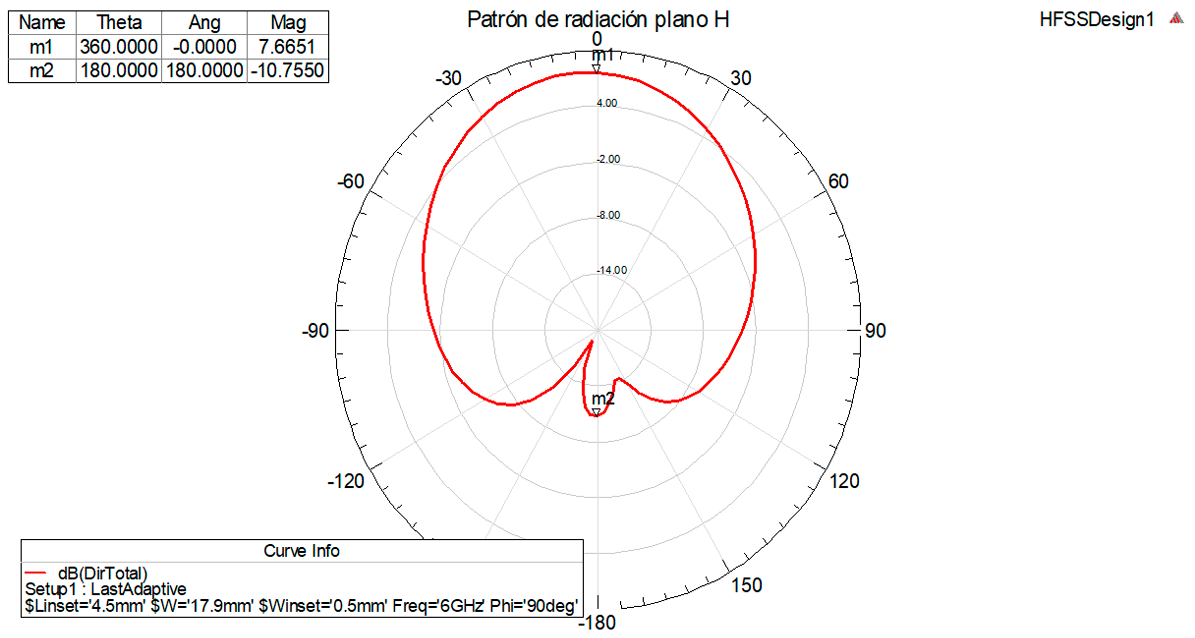
\includegraphics[width=\textwidth]{archivos/analisis/1x12/5}
        \caption{Radiación en el plano H para el parche simple a 6 GHz}
        \label{fig:H1x12}
\end{figure}

\subsection{Radiación 3D}
\par Mediante el diagrama de radiación 3D se puede observar el comportamiento omnidireccional de la antena. 

\begin{figure}[H]
     \centering
     \begin{subfigure}[b]{0.6\textwidth}
         \centering
         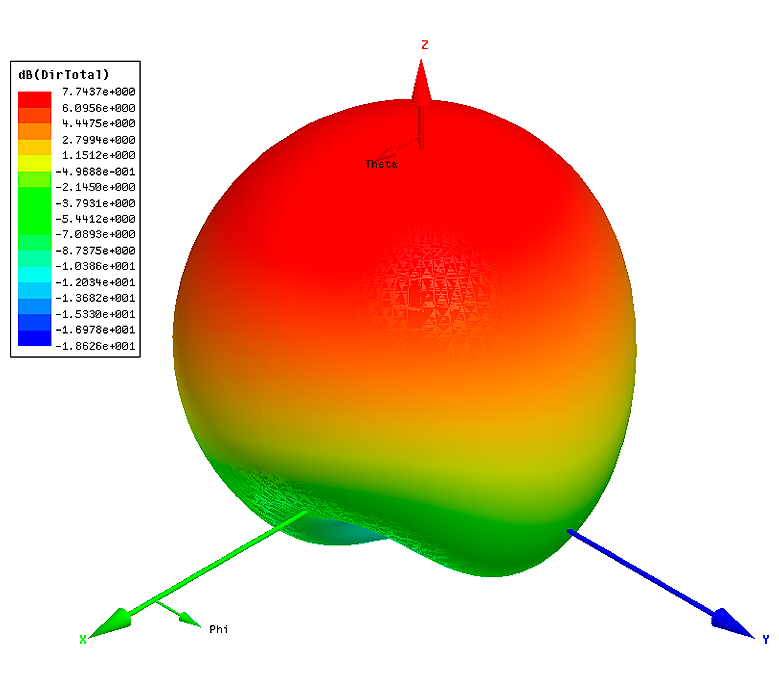
\includegraphics[width=\textwidth]{archivos/analisis/1x12/6}
         \caption{Representación isométrica del diagrama de radiación 3D}
         \label{fig:3d11x12}
     \end{subfigure}
     \hfill
     \begin{subfigure}[b]{0.6\textwidth}
         \centering
         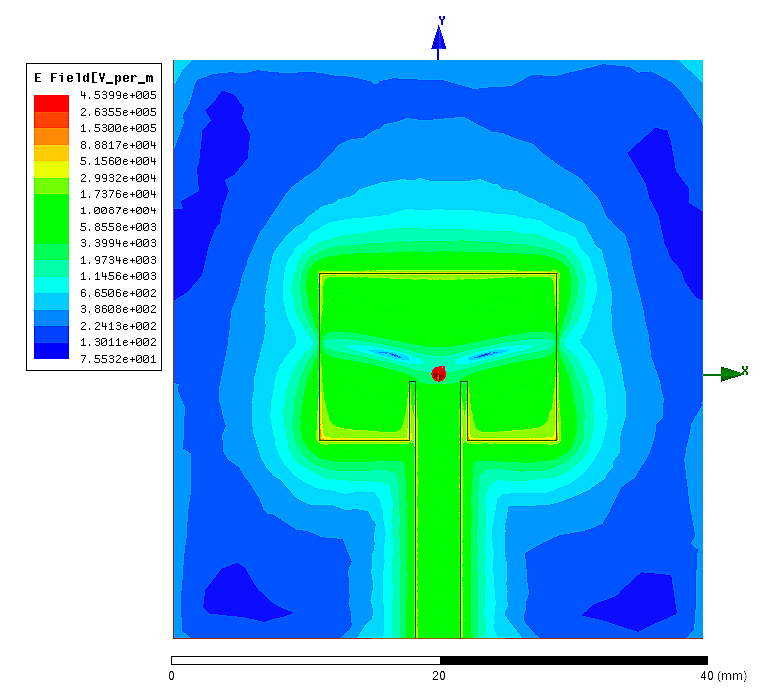
\includegraphics[width=\textwidth]{archivos/analisis/1x12/7}
         \caption{Representación superior del diagrama de radiación 3D}
         \label{fig:3d21x12}
     \end{subfigure}
     \hfill
        \caption{Radiación 3D para el parche simple a 6 GHz}
        \label{fig:3d1x12}
\end{figure}

\subsection{Campo eléctrico}
\par Finalmente, podemos observar la distribución de campos eléctricos en el parche. 

\begin{figure}[H]
    \centering
        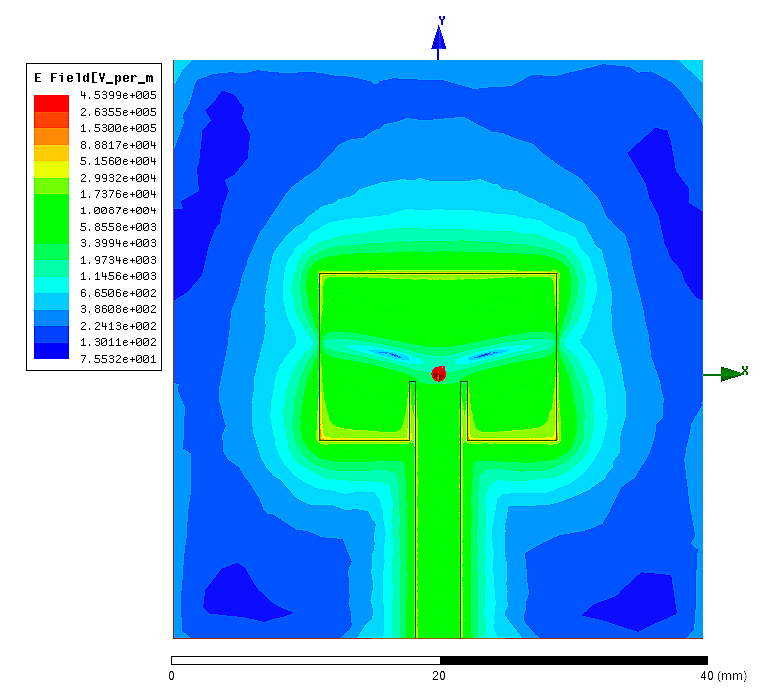
\includegraphics[width=\textwidth]{archivos/analisis/1x12/8}
        \caption{Distribución de campos eléctricos para el parche simple a 6 GHz}
        \label{fig:elec1x12}
\end{figure}









